\documentclass[conference]{IEEEtran}
\IEEEoverridecommandlockouts

\usepackage{cite}
\usepackage{amsmath,amssymb,amsfonts}
\interdisplaylinepenalty=2500
\usepackage{bm}
\usepackage{mathtools}
\usepackage{graphicx}
\usepackage{textcomp}
\usepackage{xcolor}
\usepackage{booktabs}
\usepackage{array}
\usepackage{multirow}
\usepackage{siunitx}
\usepackage{algorithm}
\usepackage{algpseudocode}
\usepackage[hidelinks]{hyperref}
\usepackage{balance}
\usepackage{tikz}
\usetikzlibrary{arrows.meta}

\graphicspath{{figures/}}

\sisetup{
    mode=match,
    propagate-math-font=true,
    reset-math-version=false,
    reset-text-family=false,
    reset-text-series=false,
    reset-text-shape=false,
    text-family-to-math=true,
    text-series-to-math=true,
    round-mode=places,
    round-precision=3
}

\newcommand{\R}{\mathbb{R}}
\newcommand{\SE}{\mathrm{SE}}
\newcommand{\SO}{\mathrm{SO}}
\newcommand{\T}{\bm{T}}
\newcommand{\Rmat}{\bm{R}}
\newcommand{\tvec}{\bm{t}}
\newcommand{\Q}{\mathcal{Q}}
\newcommand{\Pcloud}{\mathcal{P}}
\newcommand{\C}{\mathcal{C}}
\newcommand{\w}{w}
\newcommand{\x}{\bm{x}}
\newcommand{\Tzero}{\T_{0}}
\newcommand{\Tgt}{\T_{\mathrm{gt}}}
\newcommand{\Tpgt}{\T_{\mathrm{pgt}}}
\newcommand{\Test}{\T_{\mathrm{est}}}

\begin{document}

\title{Closed-Loop Control of Weighted Point Cloud Registration Using a Learned Correspondence Model}

\author{
\IEEEauthorblockN{Amine Romdhane}
\IEEEauthorblockA{
\textit{Universit\'e du Qu\'ebec \`a Trois-Rivi\`eres (UQTR)}\\
Drummondville, QC, Canada\\
Amine.Romdhane@uqtr.ca}
}

\maketitle

\begin{abstract}
This work studies closed-loop control for weighted point cloud registration, a key operation in SLAM where scan alignment affects pose estimation and map consistency. A previously trained multilayer perceptron (MLP) predicts correspondence reliability and is used to weight rigid-transform estimation. A preliminary threshold controller is first tested, then the main method applies control directly to the transform update. At each iteration, correspondences are recomputed, weighted SVD estimates the transform, and an IMC-inspired gain filters the update. The method is evaluated on synthetic data with known ground truth and on real CAD-to-scan cases with pseudo-ground-truth transforms. MLP-weighted ICP gives the best transform accuracy on synthetic tests. On real cases, unweighted ICP performs best on average, while MLP-weighted ICP wins three of twelve cases.
\end{abstract}

\begin{IEEEkeywords}
point cloud registration, SLAM, closed-loop control, internal model control, learned weighting, ICP, weighted SVD.
\end{IEEEkeywords}

\section{Introduction}
\label{sec:introduction}

Point cloud registration is an important part of SLAM. It is used to align consecutive scans or align a scan with an existing map. The estimated transform contributes directly to the robot pose, so incorrect correspondences can lead to poor localization and inconsistent maps.

This work focuses on CAD-to-scan registration, where a measured point cloud must be aligned with a reference model. This problem has similar difficulties to scan matching in SLAM: the observed cloud can be partial, noisy, or contain points that do not belong to the reference. Repeated structures can also produce correspondences that look correct locally but lead to a wrong transform.

Classical ICP handles this problem by repeatedly matching points and estimating a new rigid transform \cite{besl1992icp}. Point-to-plane ICP improves the update by using local surface information \cite{chen1992object}, while a rigid transform can also be estimated from matched 3-D points using SVD \cite{arun1987least}.

In the previous work, an MLP was trained to predict the reliability of candidate correspondences. The predicted score was used as a continuous weight in a weighted SVD registration step. This improved the way correspondences were used, but the estimation remained one-shot: correspondences were not updated after the transform changed.

This work extends that method to an iterative closed-loop registration process. The goal is to use the learned correspondence weights while continuously updating the transform and recomputing the correspondences. A preliminary threshold-control test is first used to study the effect of the MLP score. The main method then moves the control action to the transform itself, where a filter gain controls how much of each estimated correction is applied.

\subsection{Objective}
\label{subsec:objective}

The objective is to design and evaluate a closed-loop controller for weighted point cloud registration. The controller must use the learned correspondence model and must be evaluated using transform-level metrics.

The main questions are:
\begin{itemize}
    \item Can the learned correspondence model be used inside a closed-loop registration pipeline?
    \item Does the controller improve the final transform on synthetic cases?
    \item Does the same behavior transfer to real CAD-to-scan cases?
\end{itemize}

\subsection{Main Elements}
\label{subsec:elements}

The main project elements are:
\begin{itemize}
    \item an IMC-inspired threshold controller used as a preliminary diagnostic loop;
    \item a transform-level closed-loop controller where the filter gain acts on the rigid transform update;
    \item a comparison between unweighted ICP, distance-weighted ICP, and MLP-weighted ICP;
    \item a synthetic evaluation with known ground truth;
    \item a real-case evaluation using leave-one-real-case folds and pseudo-ground-truth transforms.
\end{itemize}

\section{Problem Formulation}
\label{sec:problem_formulation}

\subsection{Rigid Registration}
\label{subsec:rigid_registration}

Let $\Q=\{\bm{q}_i\}_{i=1}^{N_s}$ be the source cloud and $\Pcloud=\{\bm{p}_j\}_{j=1}^{N_t}$ be the target cloud. The registration problem is to estimate a rigid transform $\T \in \SE(3)$ such that

\begin{equation}
    \bm{p} \approx \Rmat \bm{q} + \tvec,
    \qquad
    \Rmat \in \SO(3),
    \quad
    \tvec \in \R^3.
    \label{eq:rigid_transform}
\end{equation}

In homogeneous coordinates,

\begin{equation}
    \T =
    \begin{bmatrix}
        \Rmat & \tvec \\
        \bm{0}^{\top} & 1
    \end{bmatrix}.
    \label{eq:homogeneous_transform}
\end{equation}

The registration controller starts from an initial transform $\Tzero$ and updates it iteratively.

\subsection{Candidate Correspondences}
\label{subsec:candidate_correspondences}

At iteration $k$, the source cloud is transformed using $\T_k$. A nearest-neighbor search gives a candidate correspondence set

\begin{equation}
    \C_k =
    \left\{
    c_i = (\bm{q}_i, \bm{p}_{j(i)})
    \right\}_{i=1}^{N_c}.
    \label{eq:candidate_correspondences}
\end{equation}

Each correspondence is described by a feature vector $\x_i$. The features are based on distance, normal compatibility, descriptor distance, density ratio, and mutual-nearest-neighbor information. The MLP predicts a reliability score

\begin{equation}
    \w_i = f_{\theta}(\x_i),
    \qquad
    \w_i \in [0,1].
    \label{eq:mlp_weight}
\end{equation}

During registration, the score is used as a continuous weight. It is not treated as a perfect classification decision.

\subsection{Control Objective}
\label{subsec:control_objective}

The control objective is to reduce the alignment error of the transform. Therefore, the controlled variable is not precision, recall, or F1-score. These metrics are useful for analyzing the MLP, but they do not directly define registration quality.

For synthetic data, the ground-truth transform $\Tgt$ is known. For real data, a pseudo-ground-truth transform $\Tpgt$ is used. The transform error is measured using rotation error, translation error, RMSE, and fitness.

The combined alignment error used in the experiments is

\begin{equation}
    e_{\mathrm{align}}
    =
    \mathrm{RMSE}
    +
    e_t
    +
    0.01 e_R,
    \label{eq:alignment_error}
\end{equation}

where $e_t$ is the translation error in meters and $e_R$ is the rotation error in degrees. This scalar error is used to compare methods. The separate metrics are also reported.

\section{Control Design}
\label{sec:control_design}

\subsection{IMC-Inspired Structure}
\label{subsec:imc_structure}

Internal Model Control (IMC) uses a process model and a filter to control the response of a closed loop. In this work, the idea is adapted to registration. The learned MLP provides the correspondence reliability model, while the update filter controls how much of the estimated transform correction is applied.

The analogy is not exact. The registration process is nonlinear and discrete, and the MLP is not a complete process model. The IMC idea is nevertheless useful because it separates the model-based transform estimate from the filtering of its update. This is consistent with the role of the filter in IMC, where filtering improves robustness to model mismatch \cite{ranjan2023imc}.

\subsection{Preliminary Threshold-Control Loop}
\label{subsec:threshold_control}

The first loop controlled the MLP acceptance threshold $\tau_k$. At each iteration, correspondences with a score greater than $\tau_k$ were accepted. The control error was

\begin{equation}
    e_k =
    \max(0,\bar{r}_k-r_{\mathrm{ref}})
    +
    \max(0,a_{\min}-a_k),
    \label{eq:threshold_error}
\end{equation}

where $\bar{r}_k$ is the mean point-to-plane residual of the accepted correspondences and $a_k$ is the acceptance ratio. The threshold was updated as

\begin{equation}
    \tau_{k+1}
    =
    \mathrm{clip}
    \left(
    \tau_k
    +
    \lambda
    \Delta \tau_k,
    \tau_{\min},
    \tau_{\max}
    \right).
    \label{eq:threshold_update}
\end{equation}

The threshold response is evaluated using the integral absolute error (IAE) and integral squared error (ISE). Since the loop is discrete, they are computed as

\begin{equation}
    \mathrm{IAE}
    =
    \sum_k |e_k|,
    \qquad
    \mathrm{ISE}
    =
    \sum_k e_k^2.
    \label{eq:iae_ise}
\end{equation}

The amount of threshold variation is measured using the total variation

\begin{equation}
    \mathrm{TV}_{\tau}
    =
    \sum_k
    |\tau_{k+1}-\tau_k|.
    \label{eq:threshold_tv}
\end{equation}

This loop showed an important limitation. Small values of $\lambda$ appeared better because the threshold barely moved and the stopping condition ended the loop early. The threshold loop controlled an intermediate variable rather than the registration transform itself.

\subsection{Transform-Level Closed Loop}
\label{subsec:transform_control}

The final controller acts on the rigid transform. At iteration $k$, the current transform $\T_k$ is used to generate a new correspondence set $\C_k$. Correspondence features $\x_i$ are evaluated by the MLP, and the predicted reliability $w_i$ is associated with the same correspondence set. The pair $(\C_k,w_i)$ is then used by weighted SVD to estimate $\Test$. The update filter $Q_\lambda$ determines how much of this estimate is applied to produce $\T_{k+1}$.

The resulting structure is shown in Fig.~\ref{fig:closed_loop_pipeline}, while Algorithm~\ref{alg:transform_loop} summarizes the iteration. RMSE, fitness, rotation error, translation error, and alignment error are measured as outputs. They are used to evaluate the controller. The loop is closed by using $\T_{k+1}$ as $\T_k$ at the next iteration.

Three registration methods are compared:
\begin{itemize}
    \item unweighted ICP, where the selected correspondences have equal weight;
    \item distance-weighted ICP, where the weight decreases with correspondence distance;
    \item MLP-weighted ICP, where the learned reliability is combined with the distance weight.
\end{itemize}

For MLP-weighted ICP, the solver weight is

\begin{equation}
    w_i^{\mathrm{solver}}
    =
    \max(w_i,0.02)
    \exp\left(-\left(\frac{d_i}{\sigma}\right)^2\right),
    \label{eq:solver_weight}
\end{equation}

where $d_i$ is the correspondence distance and $\sigma$ is a distance scale.

Weighted SVD produces the transform estimate $\Test$. The filter then interpolates between the current transform and this estimate:

\begin{equation}
    \T_{k+1}
    =
    \mathrm{Interp}
    \left(
    \T_k,
    \Test,
    \lambda
    \right).
    \label{eq:transform_filter}
\end{equation}

The parameter $\lambda$ is therefore the controller gain in the transform loop. A small value applies only part of the estimated correction. A value close to $1$ applies most of it.

\begin{algorithm}[t]
\caption{Transform loop}
\label{alg:transform_loop}
\begin{algorithmic}[1]
\State Initialize $\T_0$
\For{$k = 0$ to $N_{\mathrm{iter}}$}
    \State Transform the source cloud using $\T_k$
    \State Find nearest-neighbor correspondences
    \State Compute correspondence features
    \State Predict MLP reliability scores
    \State Compute solver weights
    \State Estimate $\Test$ using weighted SVD
    \State Compute $\T_{k+1}$ using $Q_\lambda$
    \State Measure RMSE, fitness, $e_R$, and $e_t$
\EndFor
\end{algorithmic}
\end{algorithm}

\begin{figure*}[t]
\centering
\resizebox{0.93\textwidth}{!}{%
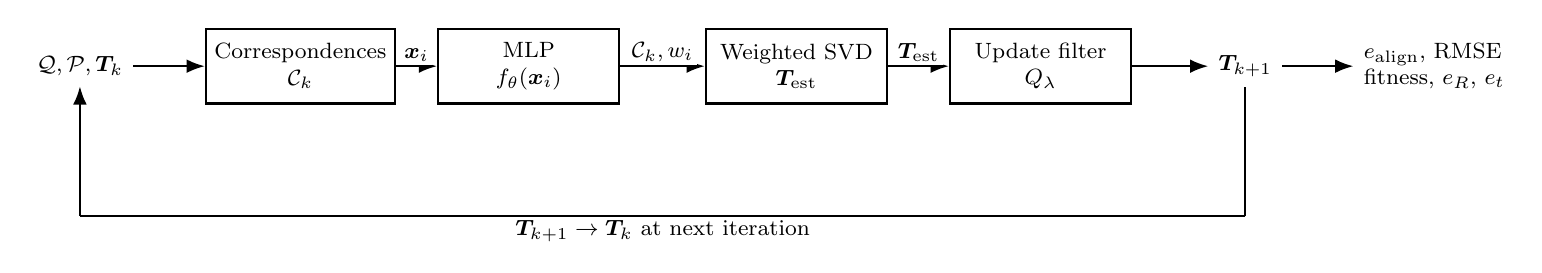
\begin{tikzpicture}[
    >=Latex,
    thick,
    font=\footnotesize,
    block/.style={
        rectangle,
        draw,
        align=center,
        minimum height=0.95cm,
        minimum width=2.30cm,
        inner sep=3pt
    },
    arrowlabel/.style={
        fill=white,
        inner sep=1.2pt
    }
]

\node[align=center] (input) at (0,0)
{$\Q,\Pcloud,\T_k$};

\node[block] (corr) at (2.8,0)
{Correspondences\\$\C_k$};

\node[block] (mlp) at (5.7,0)
{MLP\\$f_\theta(\x_i)$};

\node[block] (svd) at (9.1,0)
{Weighted SVD\\$\Test$};

\node[block] (filter) at (12.2,0)
{Update filter\\$Q_\lambda$};

\node[align=center] (update) at (14.8,0)
{$\T_{k+1}$};

\node[align=left] (metrics) at (17.2,0)
{$e_{\mathrm{align}}$, RMSE\\
fitness, $e_R$, $e_t$};

\draw[->]
(input) -- (corr);

\draw[->]
(corr) --
node[midway, above, arrowlabel] {$\x_i$}
(mlp);

\draw[->]
(mlp) --
node[midway, above, arrowlabel] {$\C_k,w_i$}
(svd);

\draw[->]
(svd) --
node[midway, above, arrowlabel] {$\Test$}
(filter);

\draw[->]
(filter) -- (update);

\draw[->]
(update) -- (metrics);

\coordinate (returnRight) at (14.8,-1.90);
\coordinate (returnLeft) at (0,-1.90);

\draw
(update.south) -- (returnRight);

\draw
(returnRight) --
node[midway, below, arrowlabel]
{$\T_{k+1}\rightarrow\T_k$ at next iteration}
(returnLeft);

\draw[->]
(returnLeft) -- (input.south);

\end{tikzpicture}%
}
\caption{Transform loop.}
\label{fig:closed_loop_pipeline}
\end{figure*}

\section{Data and Experimental Setup}
\label{sec:experimental_setup}

\subsection{Correspondence Dataset}
\label{subsec:dataset}

The correspondence dataset reused from the previous assignment contains $116278$ candidate correspondences. The target label is \texttt{target\_weight}. The dataset contains $75519$ unreliable correspondences and $40759$ reliable correspondences. The scenarios include static noise, partial overlap, strong noise, scene change, added outliers, and real previous registration cases.

The input features are:
\begin{itemize}
    \item \texttt{distance\_T0};
    \item \texttt{normal\_dot\_abs};
    \item \texttt{fpfh\_distance};
    \item \texttt{log\_normalized\_density\_ratio};
    \item \texttt{is\_mutual\_nn}.
\end{itemize}

\subsection{MLP Model}
\label{subsec:mlp_model}

The reliability model is a small MLP implemented with scikit-learn. The pipeline contains a standard scaler followed by an MLP classifier with two hidden layers:

\begin{equation}
    5 \rightarrow 32 \rightarrow 16 \rightarrow 1.
\end{equation}

The split is done by \texttt{sample\_id}, so correspondences from the same sample do not appear in both training and testing. The model gives a continuous reliability score in the final controller.

Table~\ref{tab:mlp_metrics} reports the main test metrics for two classification thresholds. The lower threshold gives higher recall, while the higher threshold gives higher precision.

\begin{table}[t]
\centering
\caption{MLP metrics.}
\label{tab:mlp_metrics}
\begin{tabular}{lcccc}
\toprule
Threshold & Accuracy & Precision & Recall & F1 \\
\midrule
0.30 & 0.588 & 0.404 & 0.819 & 0.541 \\
0.50 & 0.734 & 0.579 & 0.377 & 0.457 \\
\bottomrule
\end{tabular}
\end{table}

\subsection{Synthetic Setup}
\label{subsec:synthetic_setup}

The synthetic transform-control test uses generated asymmetric point clouds. A known transform is applied, then noise, outliers, or partial overlap are introduced depending on the scenario. The tested scenarios are clean, static noise, strong noise, partial overlap, and added outliers.

The tested gains are

\[
\lambda =
0.01,\ 0.03,\ 0.05,\ 0.10,\ 0.20,\ 0.40,\ 0.75,\ 1.00 .
\]

Each loop runs for 30 iterations. Since the ground truth is known, rotation and translation errors are measured directly.

\subsection{Real Setup}
\label{subsec:real_setup}

The real experiment uses leave-one-real-case registration examples from the previous work. Each example contains a source cloud, a target cloud, an initial transform, and a pseudo-ground-truth transform. The real errors are therefore measured relative to pseudo ground truth.

The tested gains are

\[
\lambda =
0.10,\ 0.20,\ 0.40,\ 0.75,\ 1.00 .
\]

Each loop runs for 25 iterations. RMSE, fitness, rotation error, translation error, and alignment error are evaluated.

\section{Results}
\label{sec:results}

\subsection{Threshold Control}
\label{subsec:threshold_results}

The threshold loop was tested first. In the fine sweep, very small values of $\lambda$ gave the lowest IAE and ISE. However, this result is affected by the fact that the threshold barely changes and the loop can stop after only a few iterations.

Table~\ref{tab:threshold_results} gives representative values. Fig.~\ref{fig:threshold_ise} shows the corresponding ISE trend. The result motivated the move from threshold control to transform-level control.

\begin{table}[t]
\centering
\caption{Threshold control.}
\label{tab:threshold_results}
\begin{tabular}{lcccc}
\toprule
$\lambda$ & IAE & ISE & TV$_\tau$ & F1 \\
\midrule
0.005 & \textbf{0.201} & \textbf{0.0445} & \textbf{0.00028} & \textbf{0.352} \\
0.050 & 0.681 & 0.1255 & 0.01267 & 0.344 \\
1.000 & 2.584 & 0.5628 & 0.34291 & 0.258 \\
\bottomrule
\end{tabular}
\end{table}

\begin{figure}[t]
    \centering
    
\includegraphics[width=0.95\columnwidth]
    {fig_05_global_ise_vs_lambda.png}
    \caption{Threshold ISE.}
    \label{fig:threshold_ise}
\end{figure}

\subsection{Synthetic Results}
\label{subsec:synthetic_results}

The synthetic transform experiment gives a clearer result because the final transform can be compared with known ground truth.

Table~\ref{tab:synthetic_best} reports the best tested configuration for each method. MLP-weighted ICP gives the lowest alignment error, rotation error, and translation error among the best configurations.

The gain sweep is shown in Fig.~\ref{fig:synthetic_rmse} and Fig.~\ref{fig:synthetic_align}. Fig.~\ref{fig:synthetic_rmse} shows the nearest-neighbor RMSE, while Fig.~\ref{fig:synthetic_align} shows the transform-level alignment error.

\begin{table*}[t]
\centering
\caption{Synthetic results.}
\label{tab:synthetic_best}
\begin{tabular}{lcccccc}
\toprule
Method & $\lambda$ & RMSE & Fitness & Rot. err. &
Trans. err. & Align. err. \\
\midrule
Distance-weighted ICP
& 1.00 & 0.0310 & \textbf{0.9396}
& 0.376$^{\circ}$ & 0.00537 m & 0.0402 \\

MLP-weighted ICP
& 0.75 & 0.0320 & 0.9394
& \textbf{0.196$^{\circ}$}
& \textbf{0.00246 m}
& \textbf{0.0365} \\

Unweighted ICP
& 1.00 & \textbf{0.0294} & 0.8961
& 0.620$^{\circ}$ & 0.01856 m & 0.0541 \\
\bottomrule
\end{tabular}
\end{table*}

Unweighted ICP obtains the lowest nearest-neighbor RMSE in Table~\ref{tab:synthetic_best} and Fig.~\ref{fig:synthetic_rmse}, but its fitness and transform errors are worse. RMSE alone is therefore not sufficient to evaluate the final pose. Fig.~\ref{fig:synthetic_align} shows that MLP-weighted ICP with $\lambda=0.75$ gives the lowest final alignment error.

\begin{figure}[t]
    \centering
    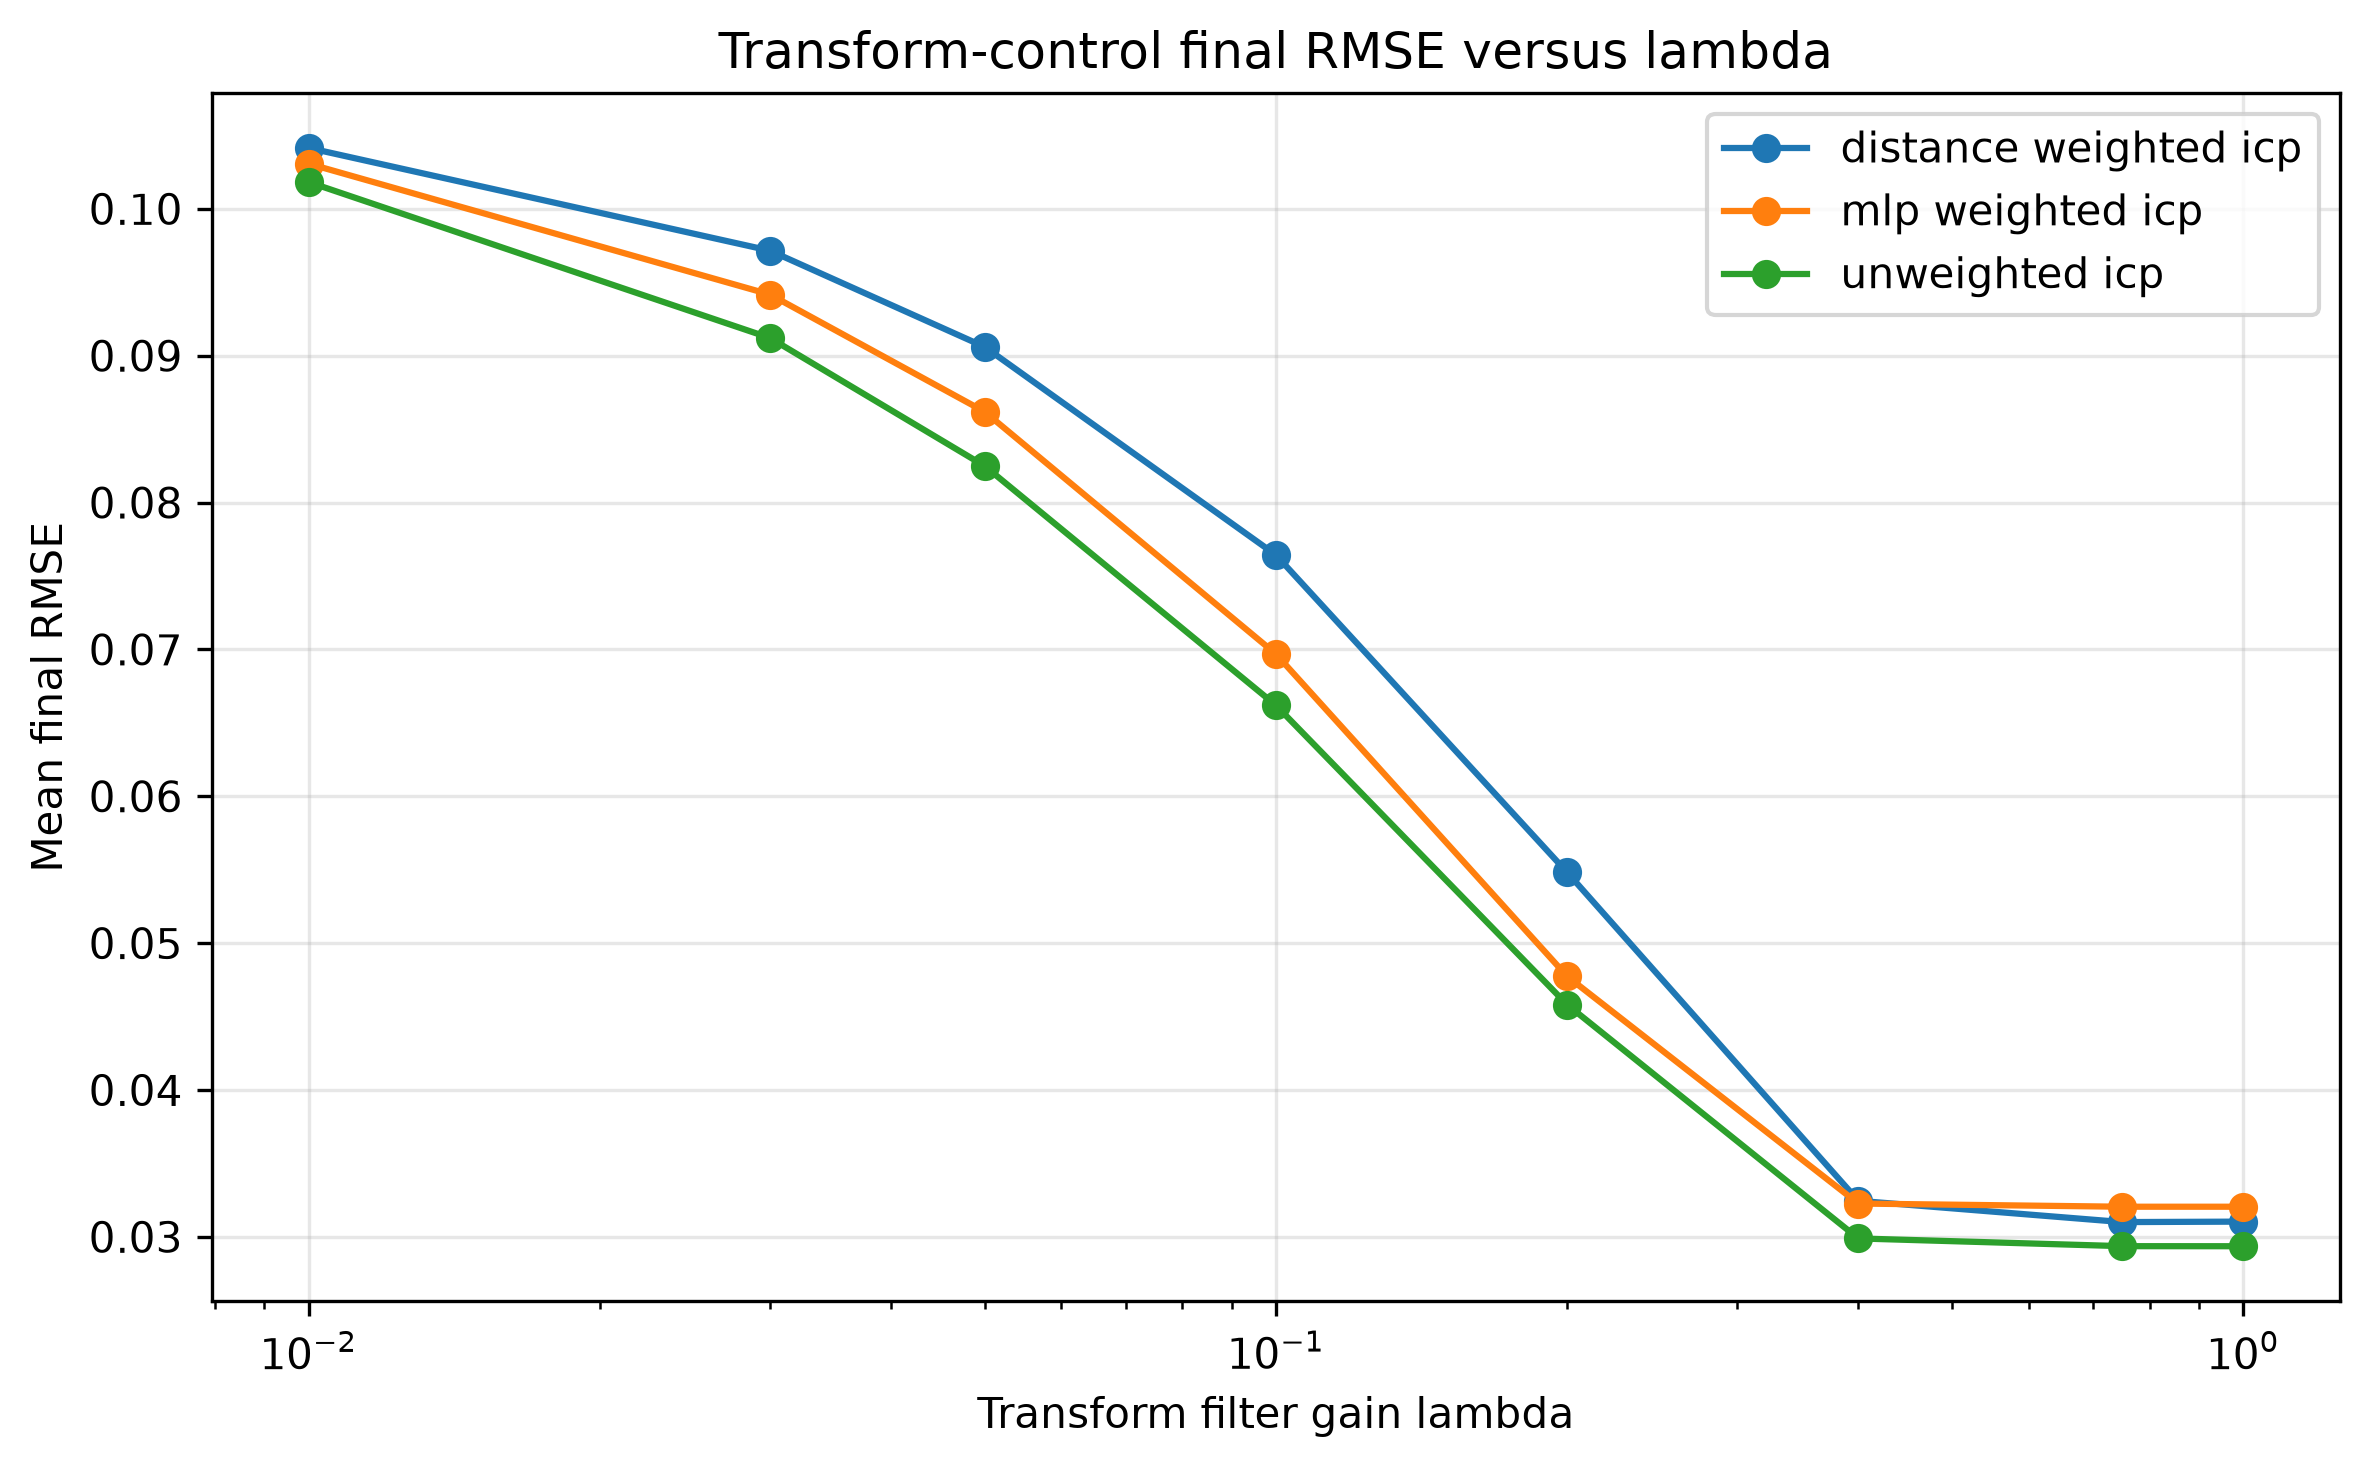
\includegraphics[width=0.95\columnwidth]
    {fig_09_transform_final_rmse_vs_lambda.png}
    \caption{Synthetic RMSE.}
    \label{fig:synthetic_rmse}
\end{figure}

\begin{figure}[t]
    \centering
    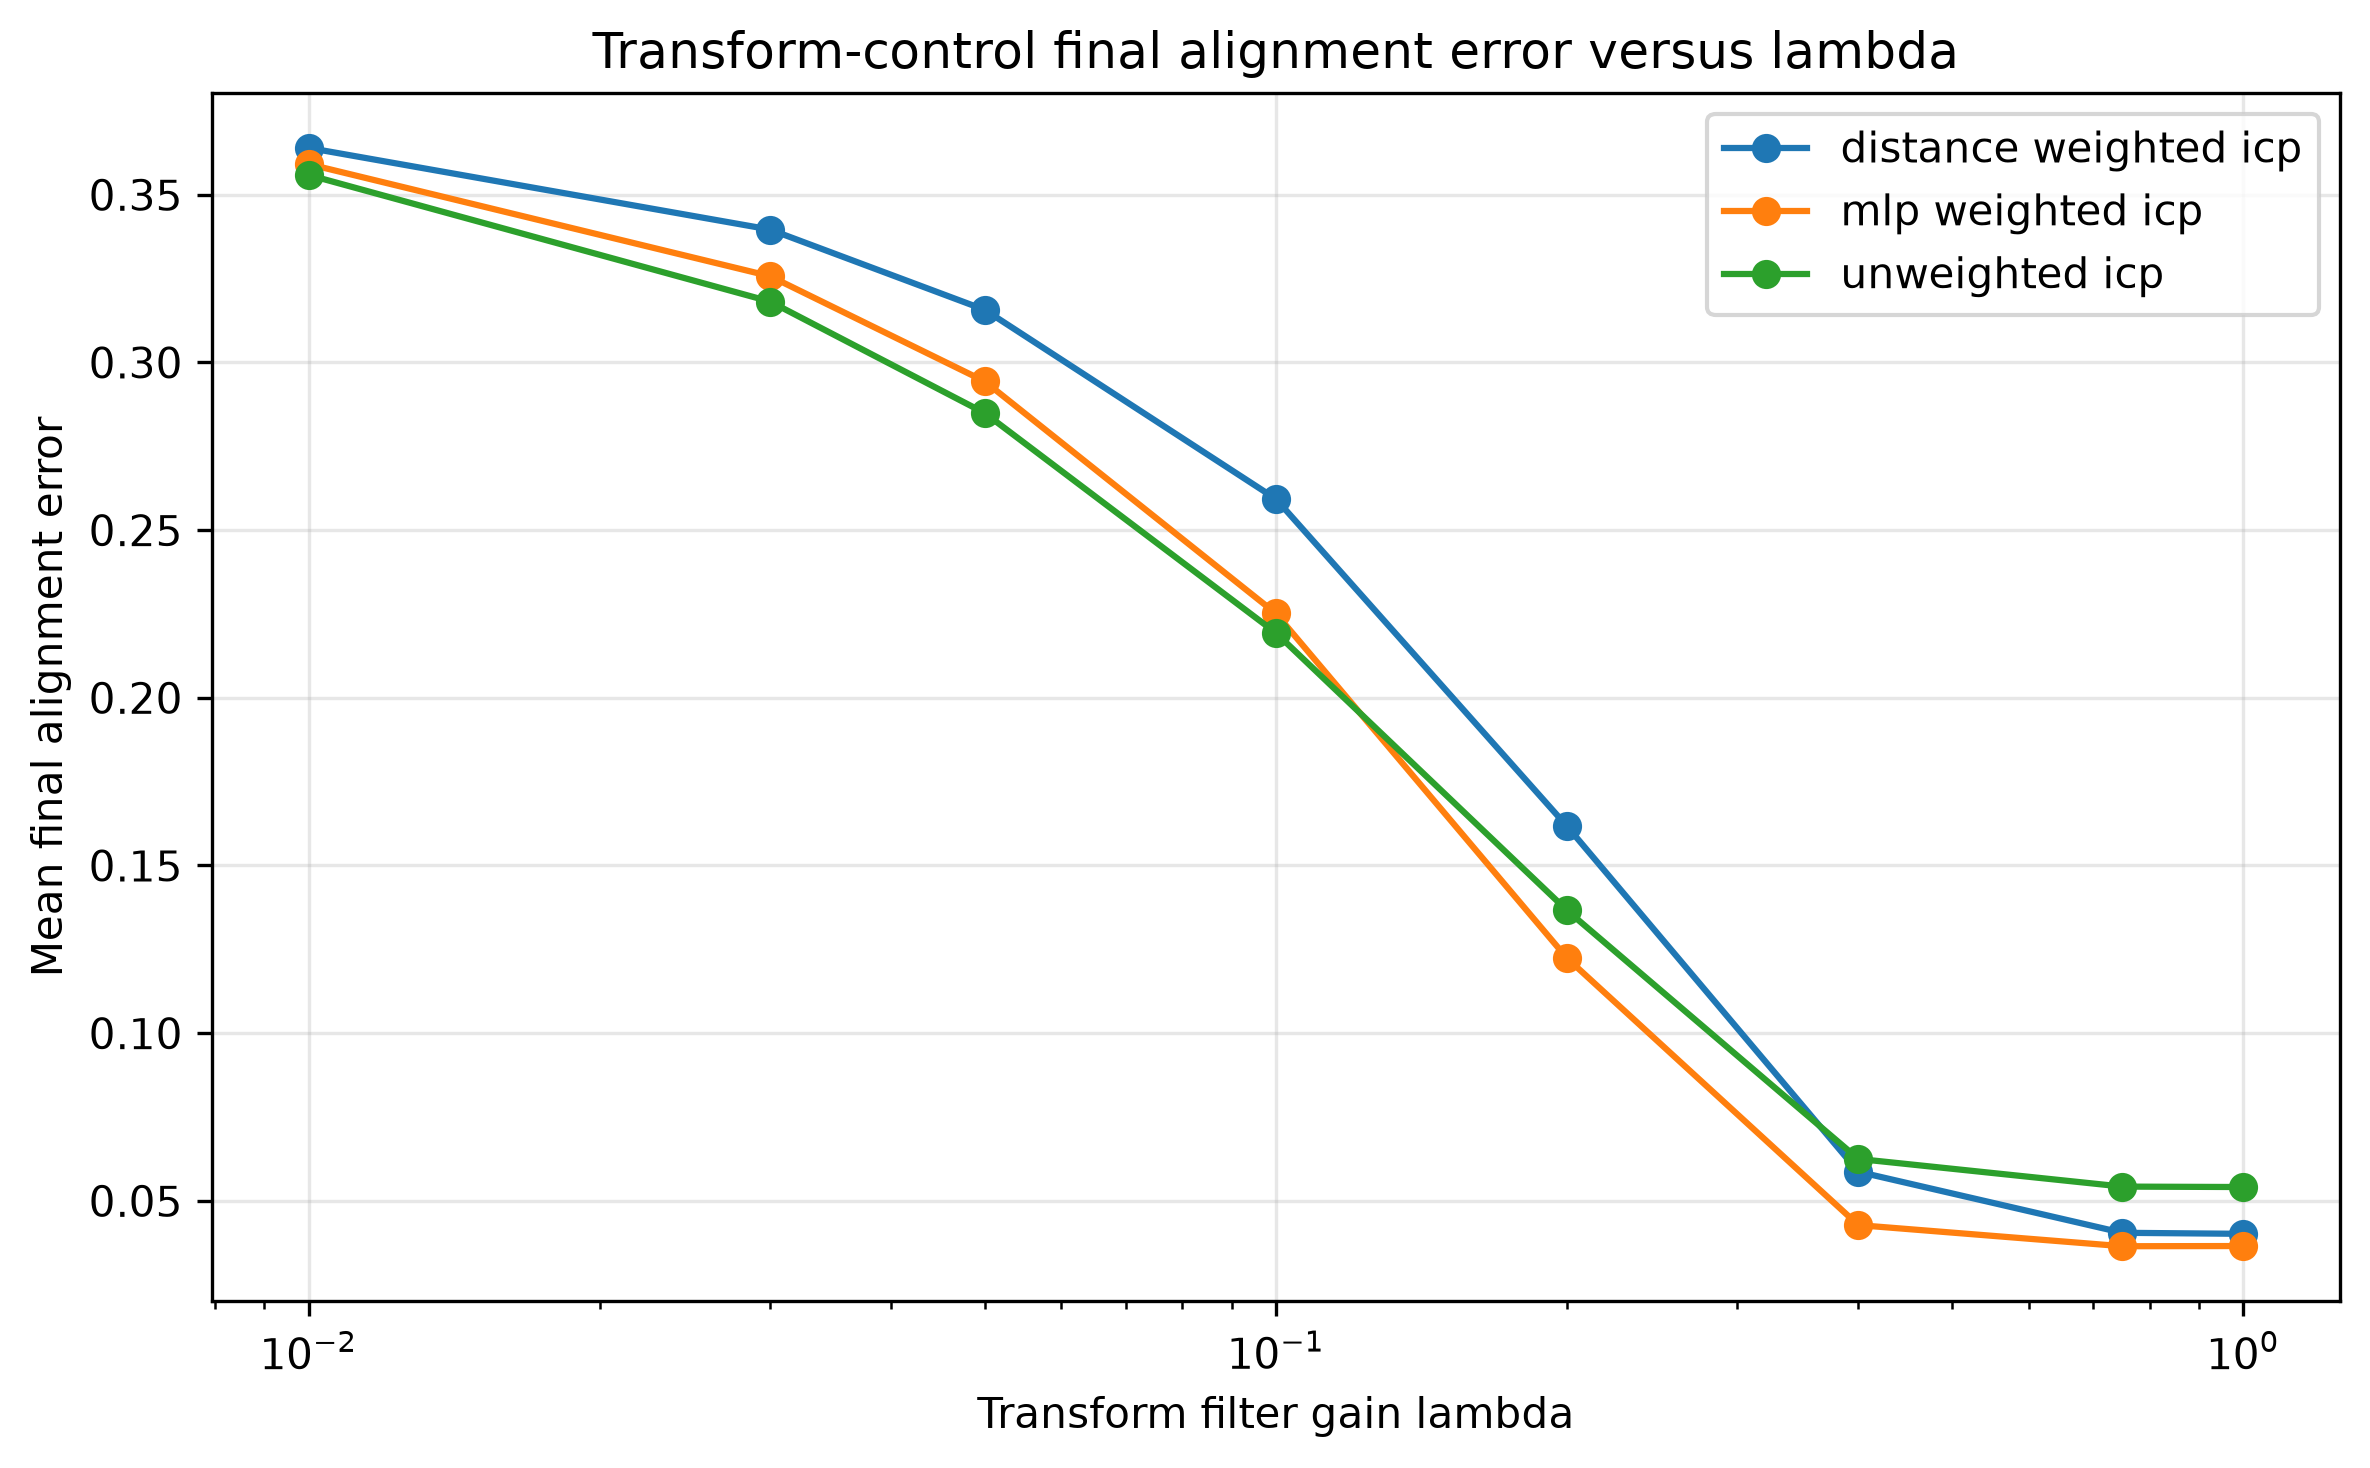
\includegraphics[width=0.95\columnwidth]
    {fig_10_transform_final_alignment_error_vs_lambda.png}
    \caption{Synthetic alignment error.}
    \label{fig:synthetic_align}
\end{figure}

\subsection{Real Results}
\label{subsec:real_results}

The real experiment gives a mixed result. Table~\ref{tab:real_best_global} reports the best average configuration for each method. Unweighted ICP gives the lowest average alignment error, while distance-weighted ICP gives the lowest average rotation error.

The real gain sweep is shown in Fig.~\ref{fig:real_align}, Fig.~\ref{fig:real_trans}, and Fig.~\ref{fig:real_rot}. The three plots separate the combined alignment, translation, and rotation errors.

\begin{table*}[t]
\centering
\caption{Real results.}
\label{tab:real_best_global}
\begin{tabular}{lcccccc}
\toprule
Method & $\lambda$ & RMSE & Fitness & Rot. err. &
Trans. err. & Align. err. \\
\midrule
Unweighted ICP
& 0.75 & \textbf{0.1027} & 0.5229
& 3.246$^{\circ}$
& \textbf{0.0986 m}
& \textbf{0.2338} \\

Distance-weighted ICP
& 1.00 & 0.1094 & \textbf{0.5319}
& \textbf{2.463$^{\circ}$}
& 0.1254 m & 0.2594 \\

MLP-weighted ICP
& 1.00 & 0.1126 & 0.5273
& 3.262$^{\circ}$
& 0.1408 m & 0.2860 \\
\bottomrule
\end{tabular}
\end{table*}

The average result does not describe every case. MLP-weighted ICP obtains the lowest alignment error in three of the twelve real cases. Table~\ref{tab:real_win_count} summarizes the winner count.

\begin{table}[t]
\centering
\caption{Real case wins.}
\label{tab:real_win_count}
\begin{tabular}{lc}
\toprule
Method & Wins \\
\midrule
Unweighted ICP & \textbf{7}/12 \\
MLP-weighted ICP & 3/12 \\
Distance-weighted ICP & 2/12 \\
\bottomrule
\end{tabular}
\end{table}

Fig.~\ref{fig:real_example} shows one real case where MLP-weighted ICP gives the lowest final alignment error. In this palletizer case, MLP-weighted ICP with $\lambda=1.0$ continues reducing the pseudo-ground-truth alignment error until the end of the loop.

\begin{figure*}[t]
    \centering
    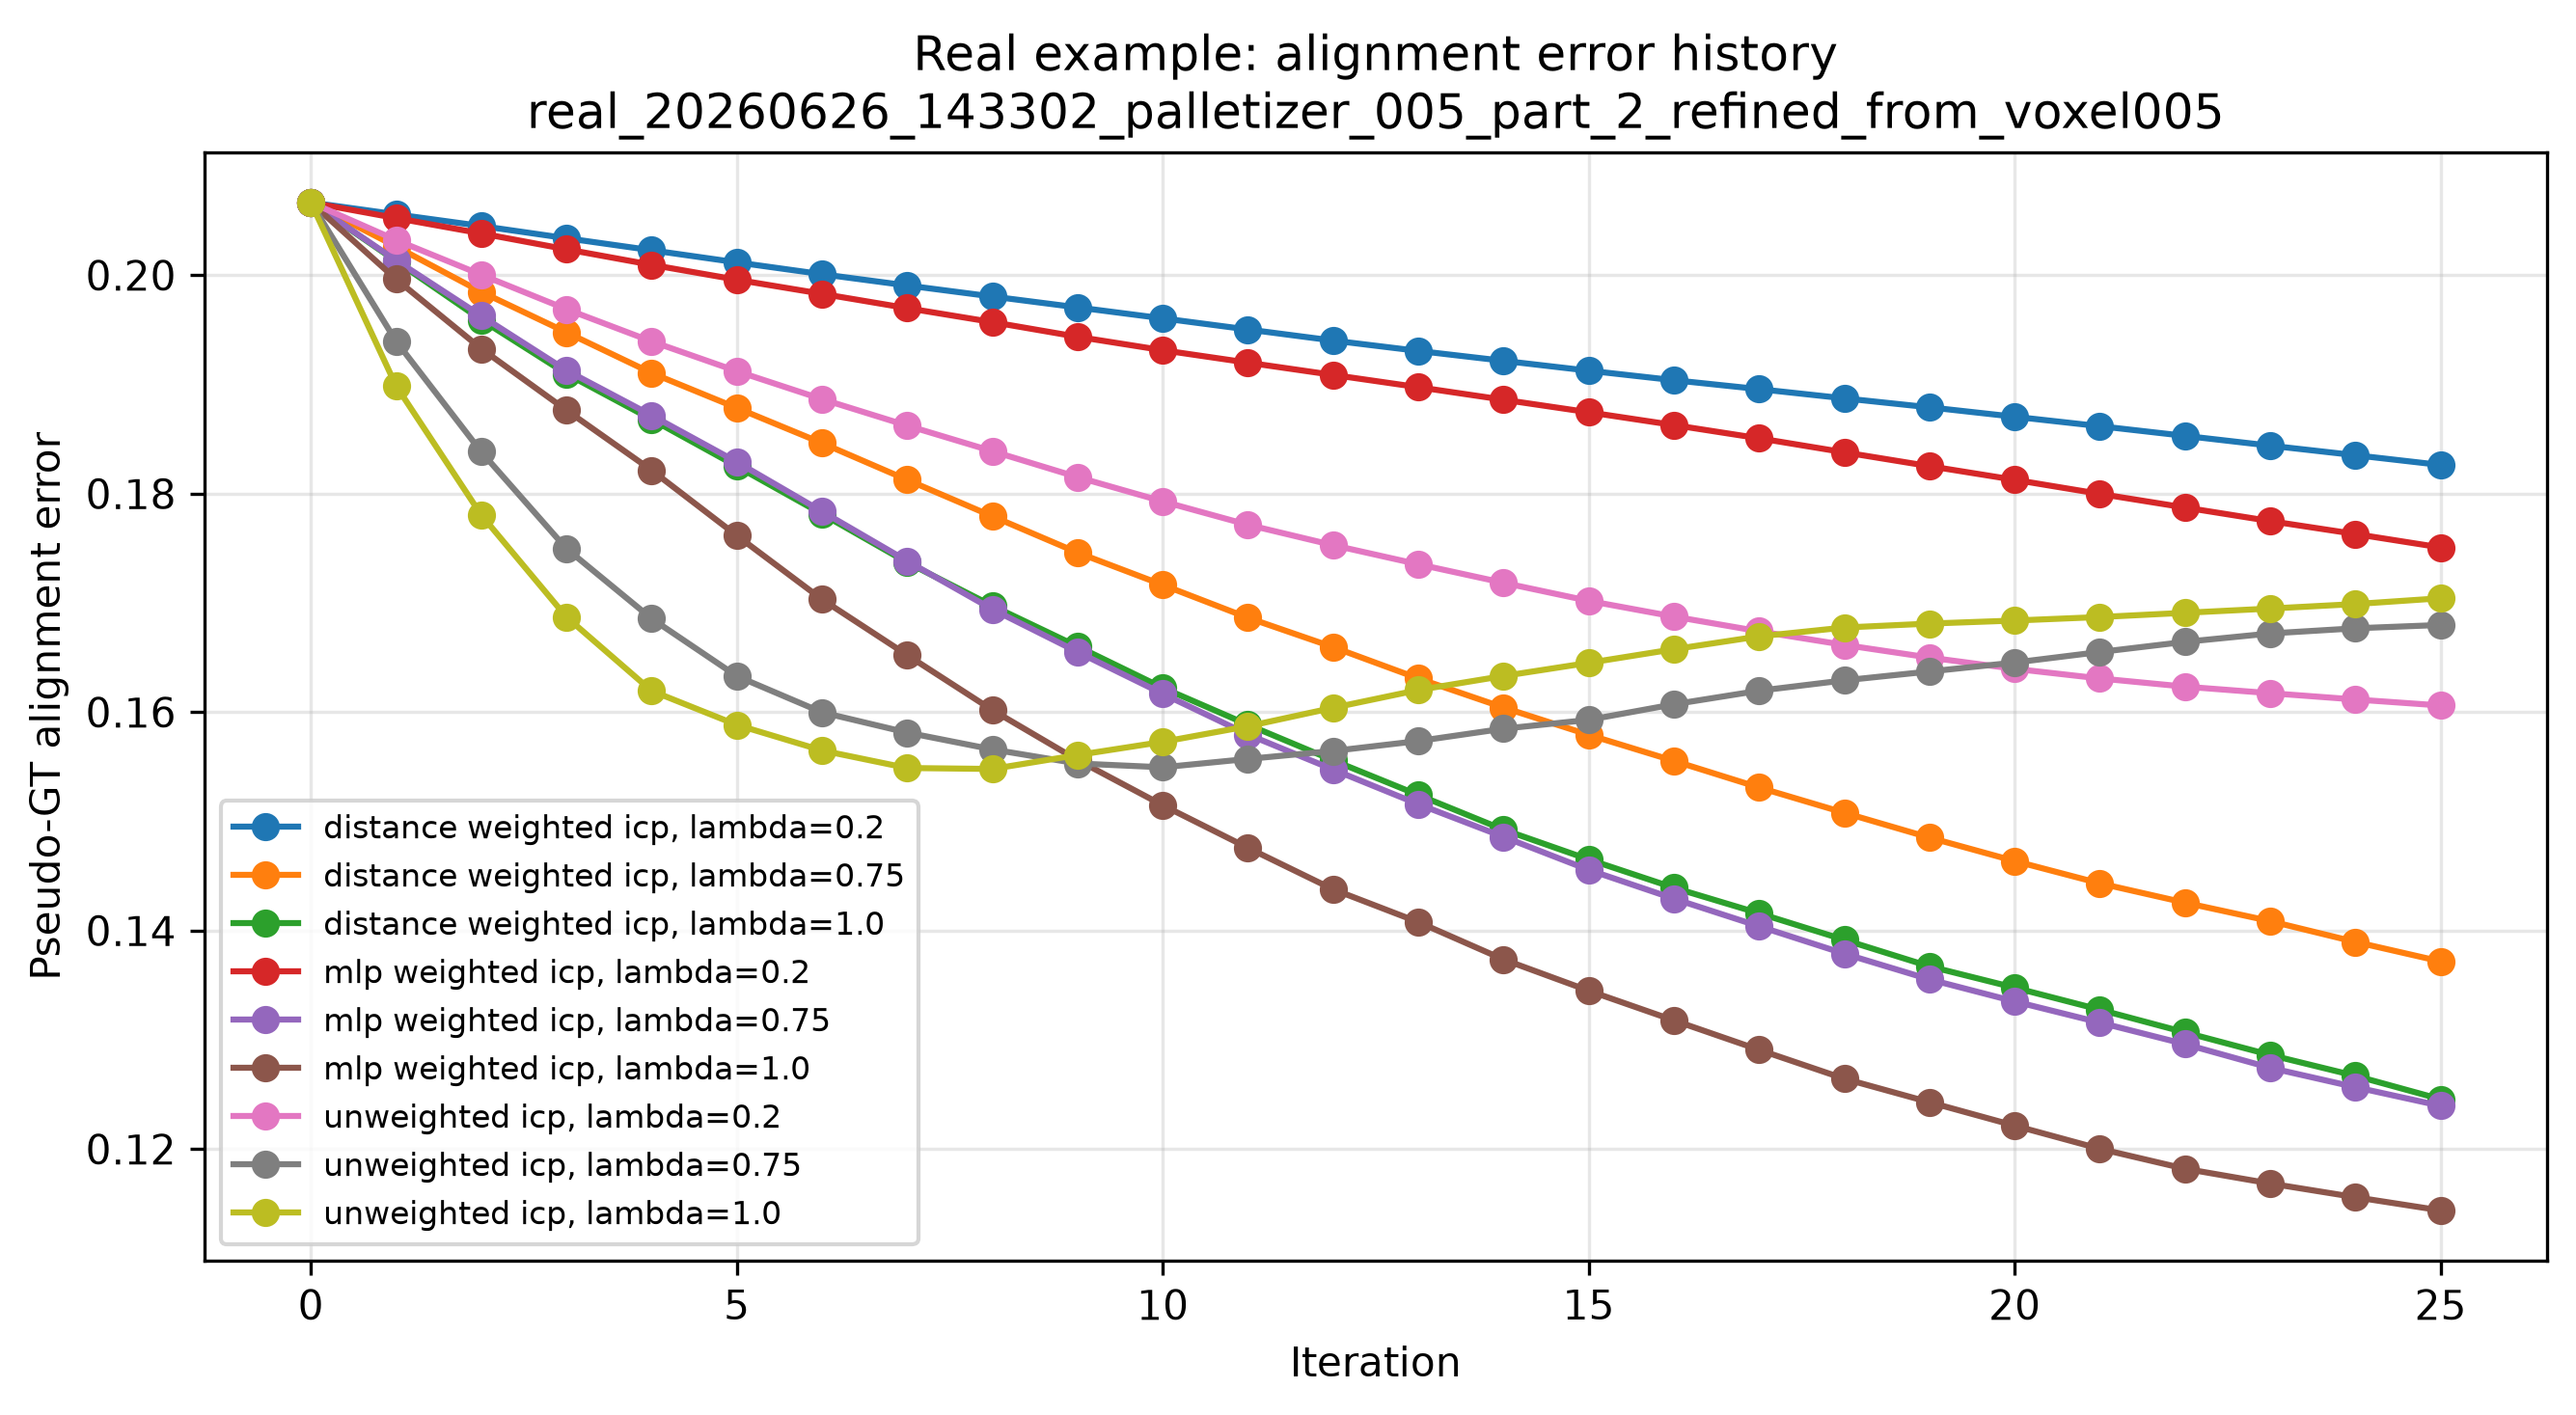
\includegraphics[width=0.85\textwidth]
    {fig_18_real_example_alignment_history.png}
    \caption{Real example.}
    \label{fig:real_example}
\end{figure*}

Fig.~\ref{fig:real_align} shows that unweighted ICP gives the lowest average combined alignment error. Fig.~\ref{fig:real_trans} shows the translation error, while Fig.~\ref{fig:real_rot} shows that distance-weighted ICP gives the lowest average rotation error.

\begin{figure}[t]
    \centering
    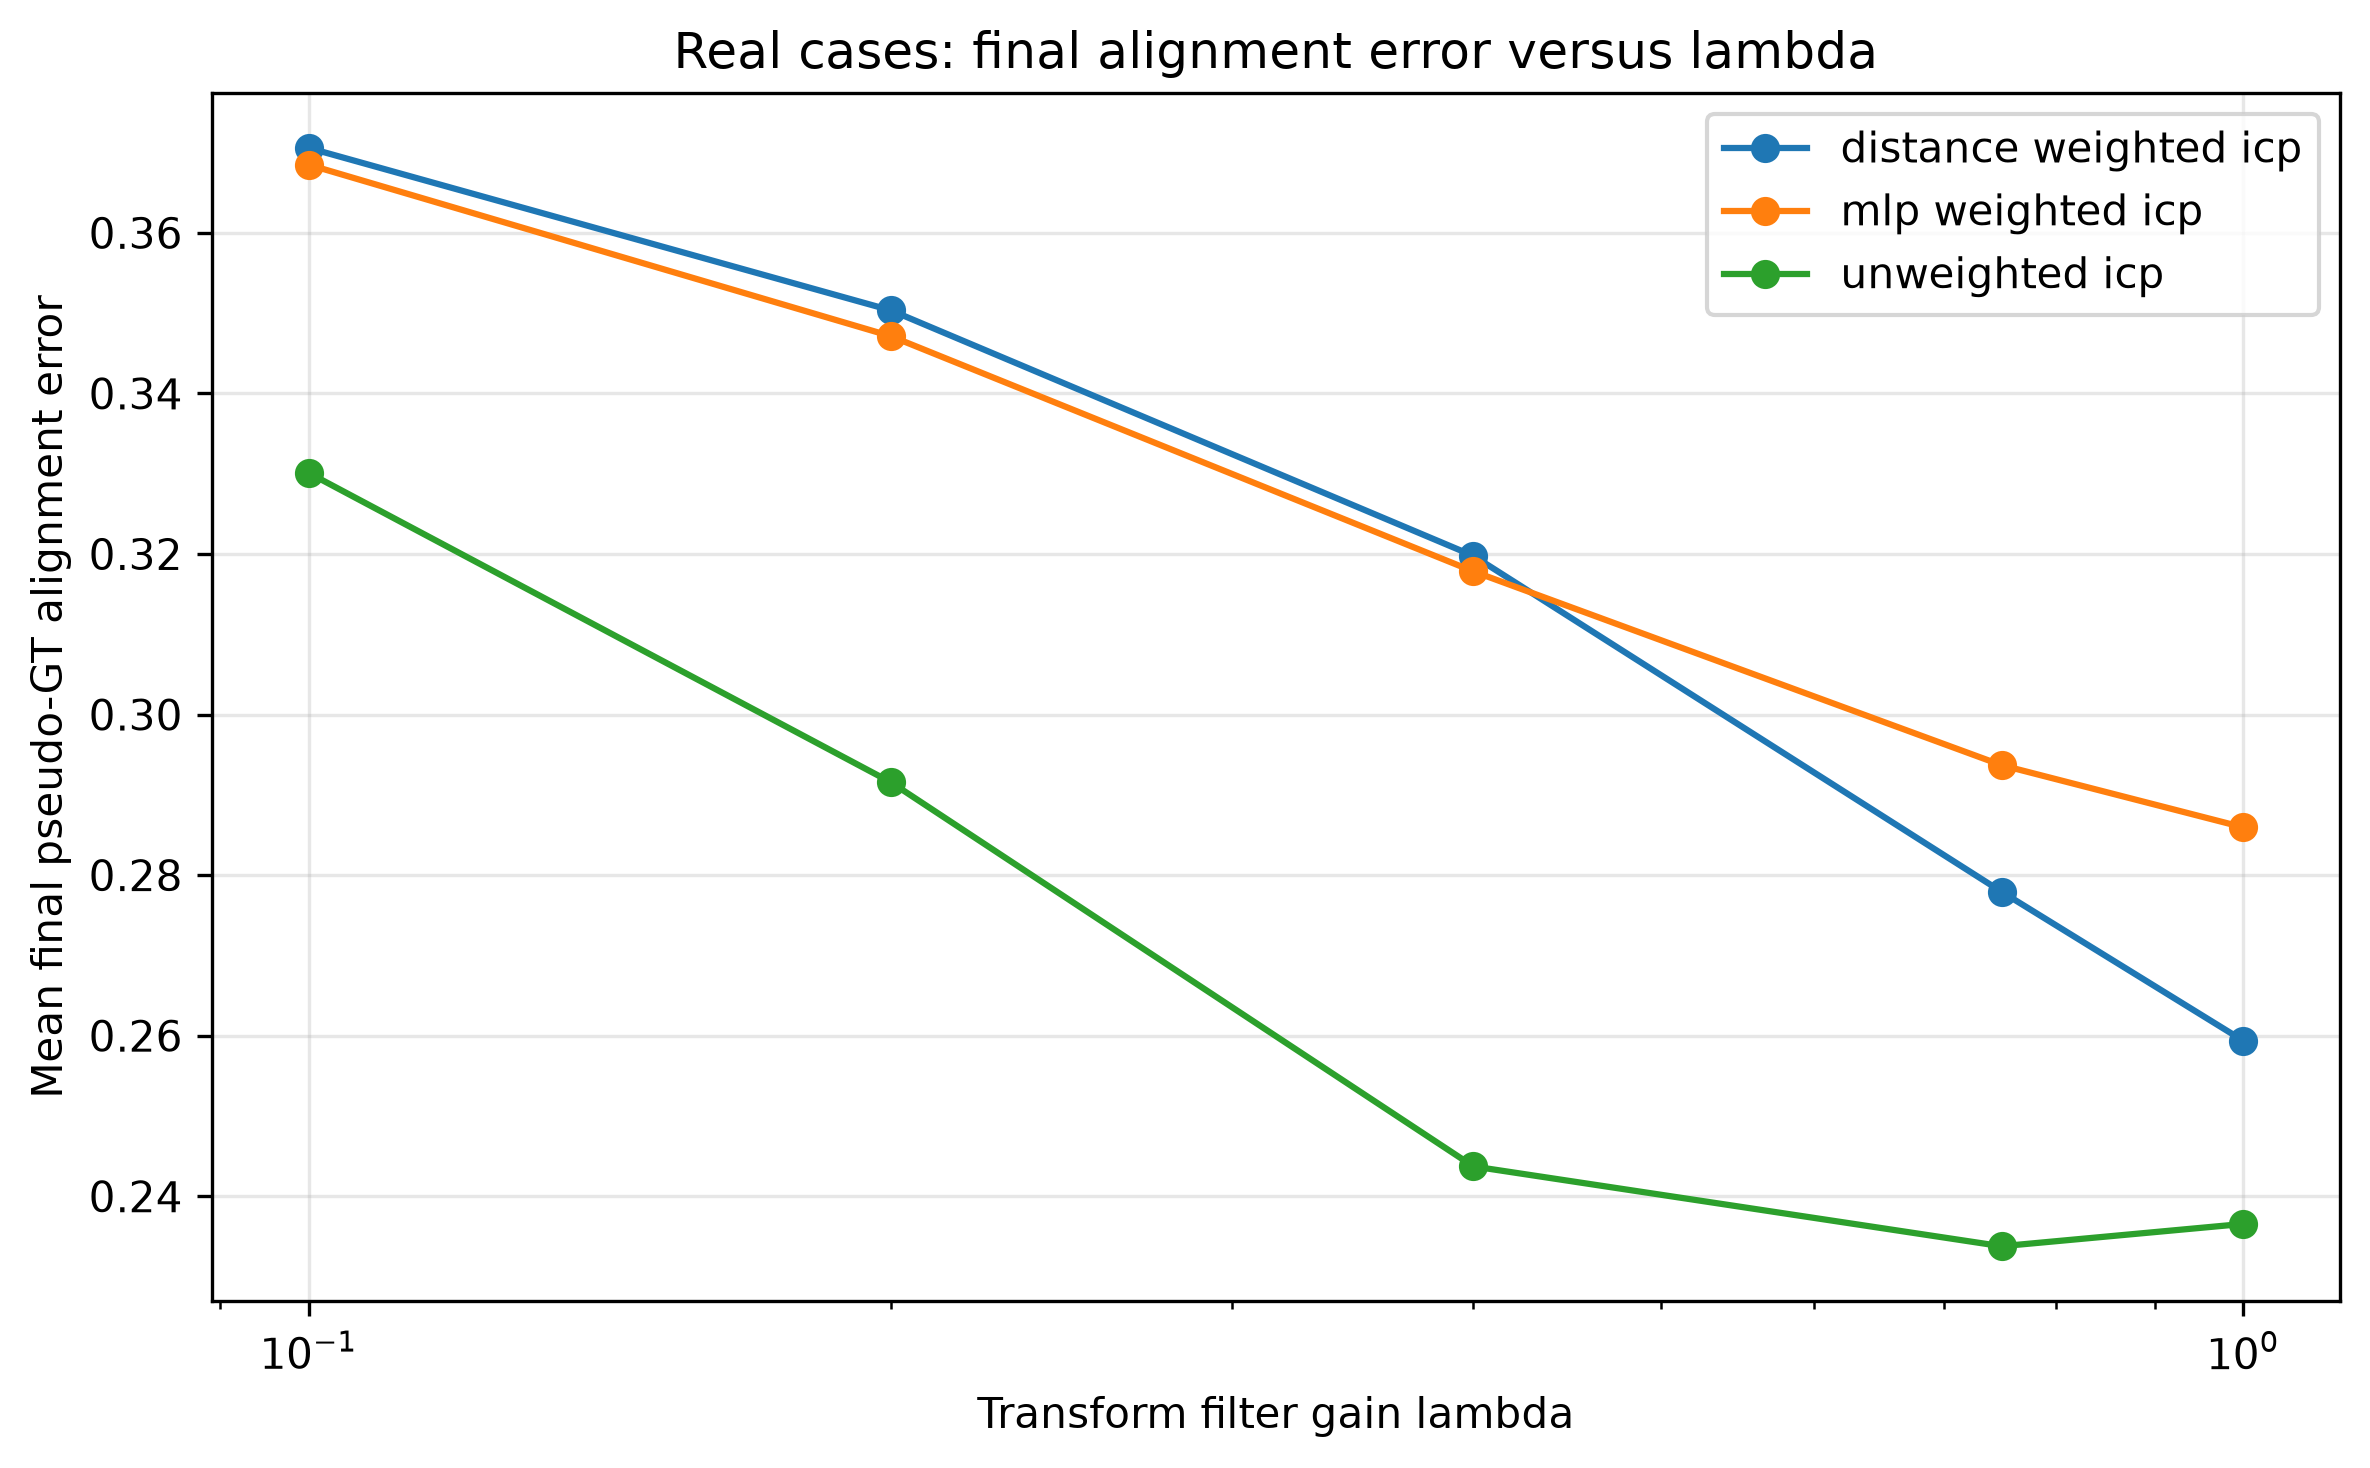
\includegraphics[width=0.95\columnwidth]
    {fig_14_real_final_alignment_error_vs_lambda.png}
    \caption{Real alignment error.}
    \label{fig:real_align}
\end{figure}

\begin{figure}[t]
    \centering
    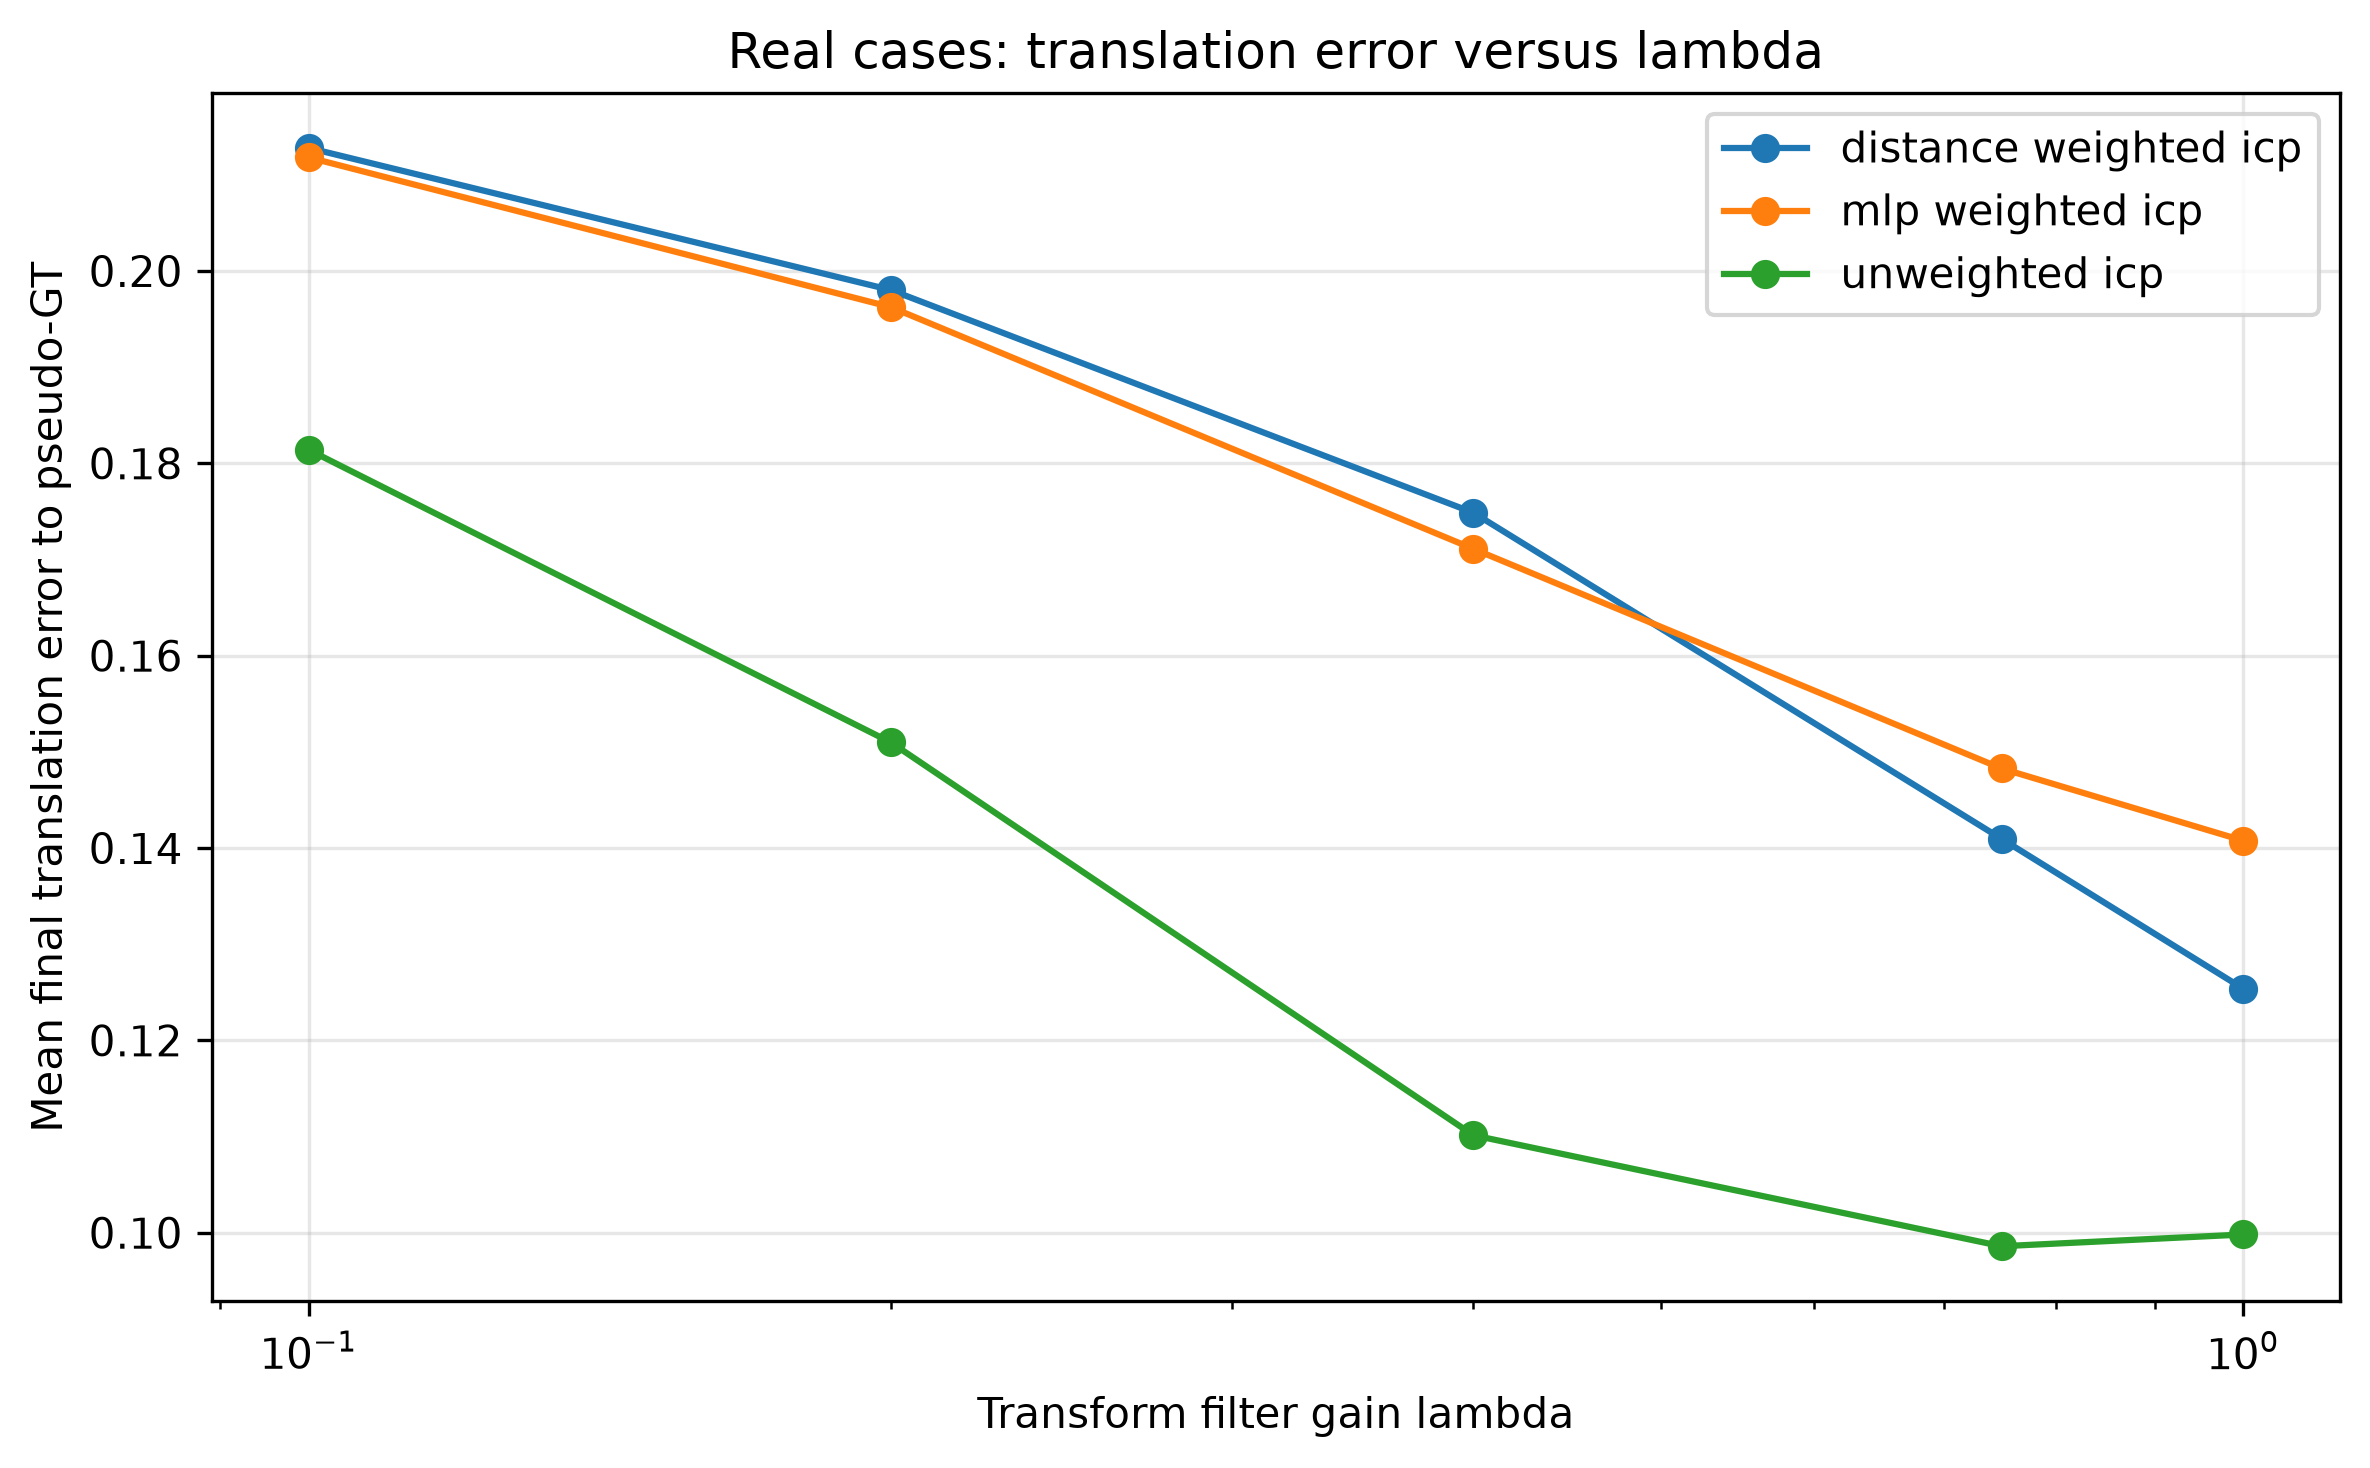
\includegraphics[width=0.95\columnwidth]
    {fig_16_real_translation_error_vs_lambda.png}
    \caption{Real translation error.}
    \label{fig:real_trans}
\end{figure}

\begin{figure}[t]
    \centering
    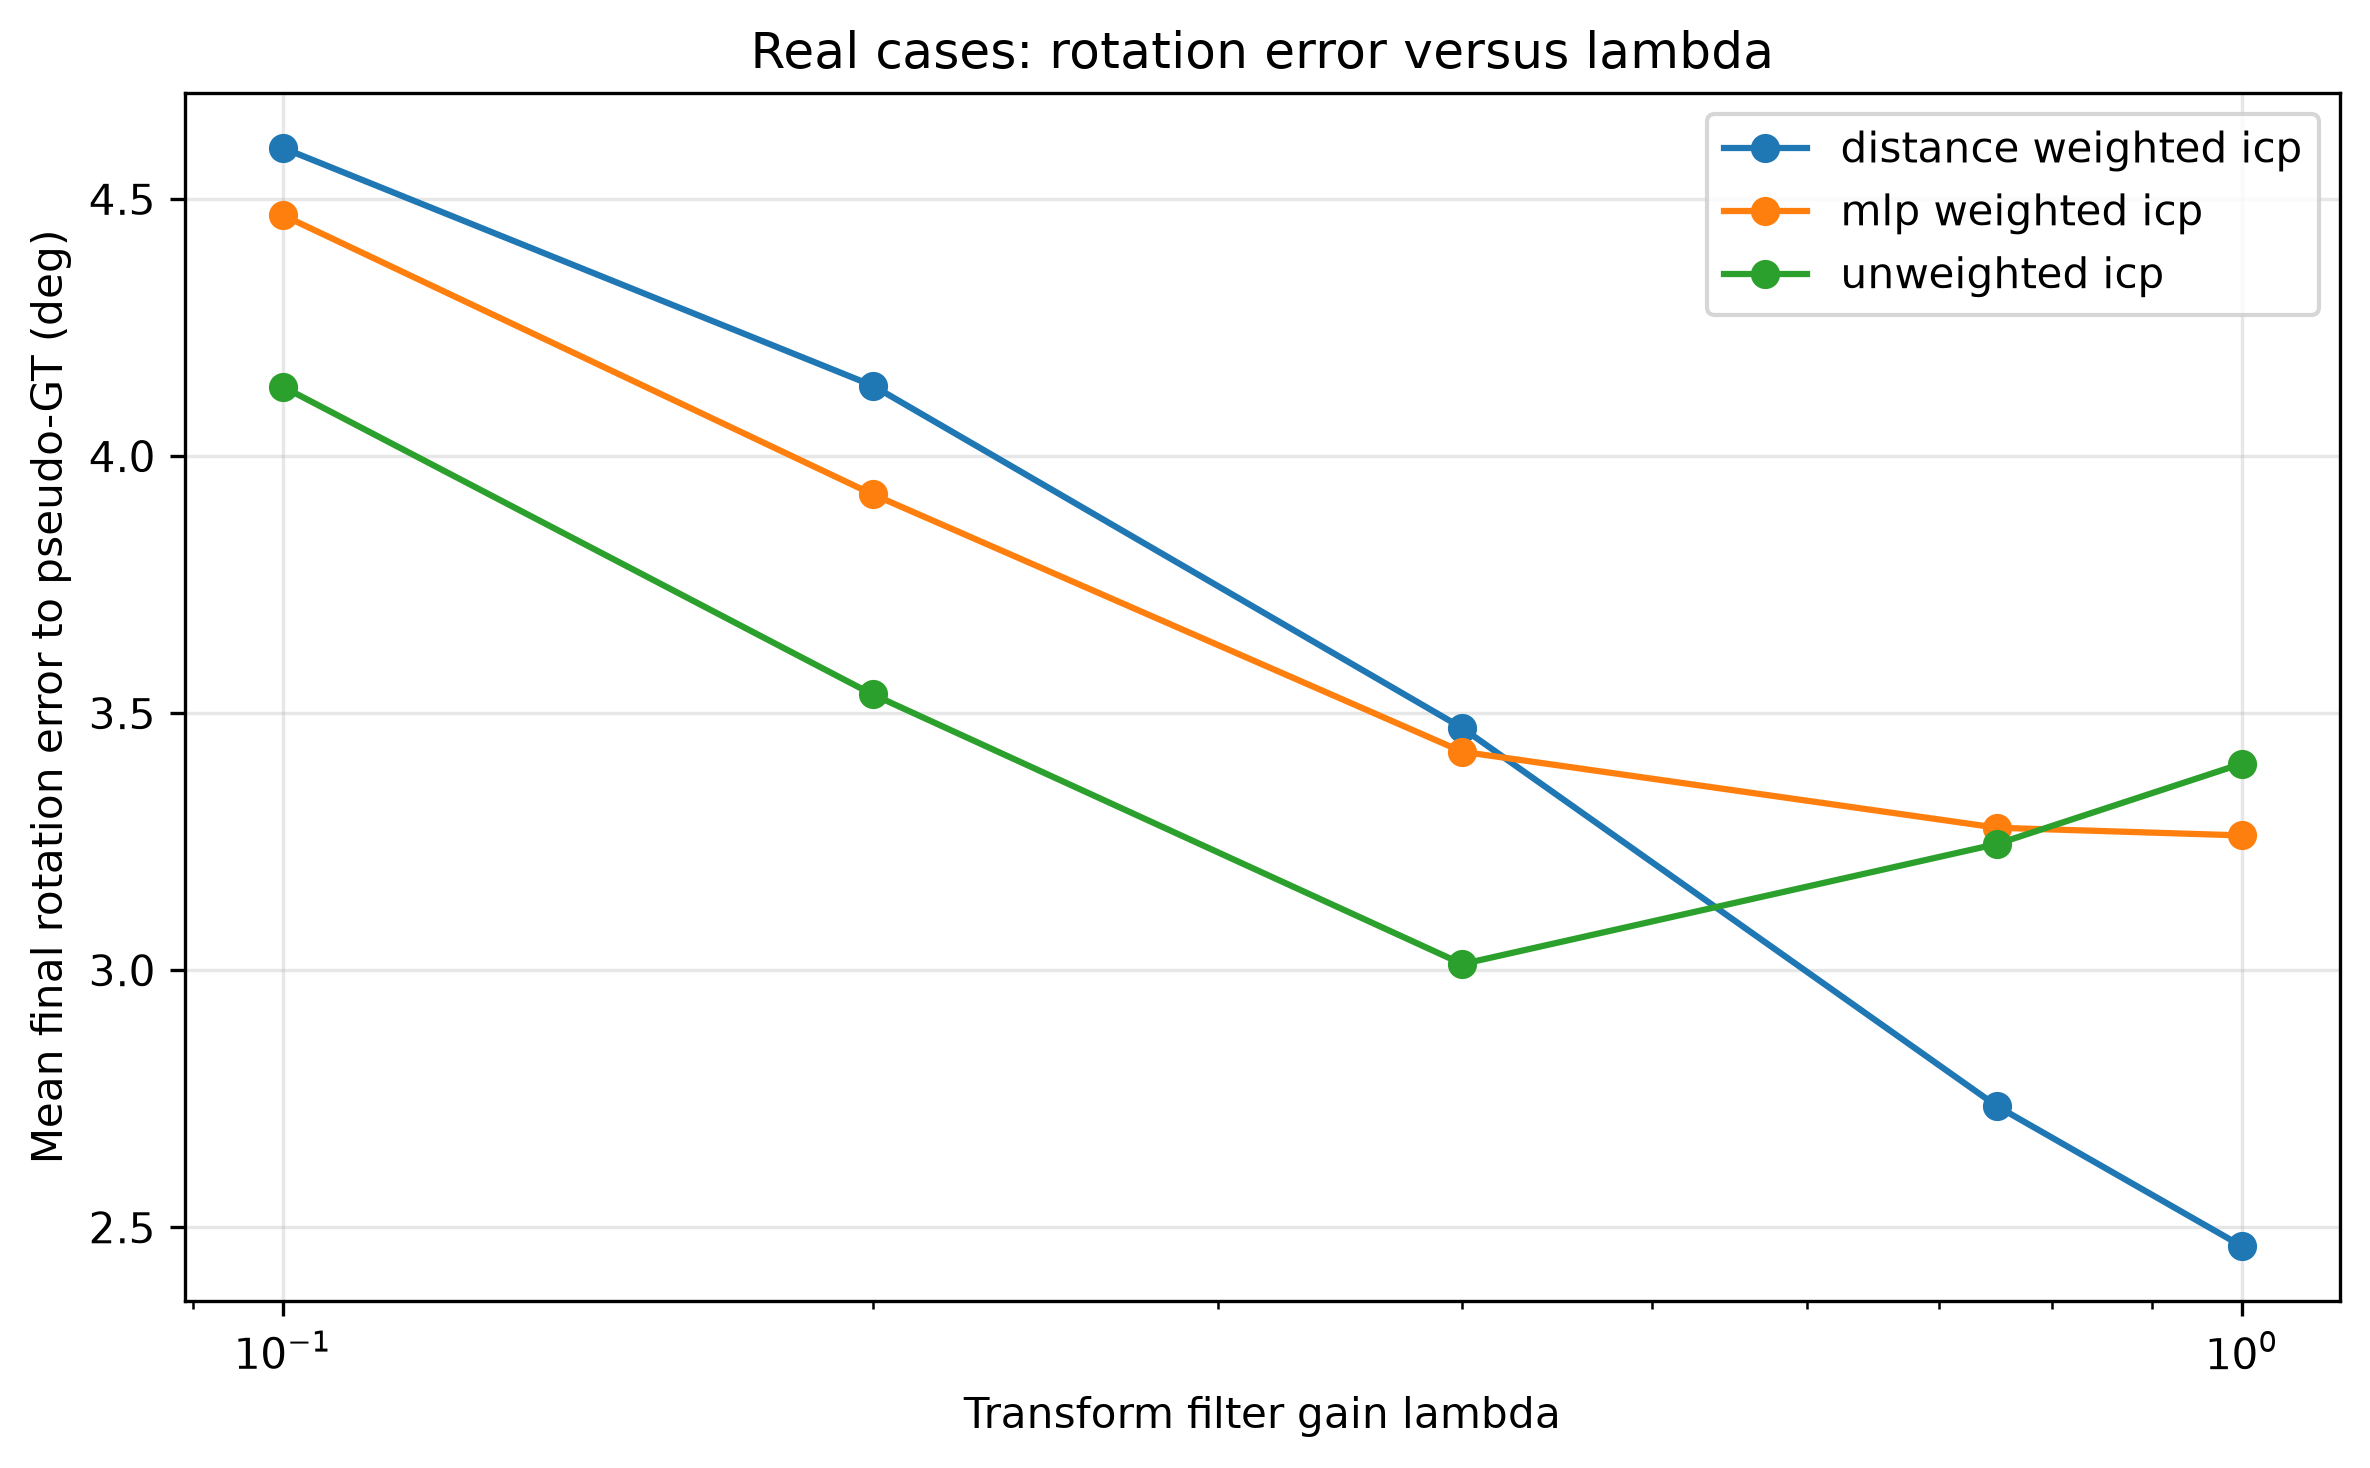
\includegraphics[width=0.95\columnwidth]
    {fig_17_real_rotation_error_vs_lambda.png}
    \caption{Real rotation error.}
    \label{fig:real_rot}
\end{figure}

\section{Discussion}
\label{sec:discussion}

\subsection{Threshold and Transform Control}
\label{subsec:threshold_vs_transform}

The threshold-control loop controls correspondence selection but not the final rigid transform. Fig.~\ref{fig:threshold_ise} also shows why very small gains can appear favorable when the threshold barely changes.

The transform loop in Fig.~\ref{fig:closed_loop_pipeline} addresses this limitation by applying the control action directly to the transform update.

\subsection{Synthetic Results}
\label{subsec:synthetic_discussion}

MLP-weighted ICP gives the lowest transform-level alignment error in Table~\ref{tab:synthetic_best} and Fig.~\ref{fig:synthetic_align}. In contrast, unweighted ICP gives the lowest nearest-neighbor RMSE in Fig.~\ref{fig:synthetic_rmse}. The difference shows that a low correspondence RMSE does not necessarily correspond to the most accurate pose.

The best tested synthetic gain for MLP-weighted ICP is $\lambda=0.75$. Applying most of the estimated correction gives the best result among the tested gains.

\subsection{Real Results}
\label{subsec:real_discussion}

The real results are less consistent. Unweighted ICP gives the best average alignment error in Table~\ref{tab:real_best_global} and Fig.~\ref{fig:real_align}, and wins seven of the twelve cases. MLP-weighted ICP wins three cases, including the example shown in Fig.~\ref{fig:real_example}.

Real CAD-to-scan registration contains partial overlap, repeated structures, segmentation errors, and CAD-scan differences. In addition, the real reference transforms are pseudo ground truth rather than physical measurements.

The learned weighting is therefore useful in some real cases, but its transfer is not consistent across the complete real set.

\subsection{Filter Gain}
\label{subsec:lambda_discussion}

The role of $\lambda$ differs between the two loops. In threshold control, it scales the threshold correction. In transform control, it scales the rigid transform update.

For the transform loop, small gains move the transform slowly. The synthetic MLP-weighted method performs best at $\lambda=0.75$, while the real MLP-winning cases use $\lambda=1.0$.

\section{Limitations}
\label{sec:limitations}

The limitation is the pseudo-ground-truth reference used for the real cases. The reported real rotation and translation errors are therefore relative to a previous registration result.

The MLP also evaluates correspondences independently. Global rigid consistency only enters later through weighted SVD.

Finally, the real dataset contains a limited number of object-specific cases.

\section{Conclusion}
\label{sec:conclusion}

A closed-loop registration controller was implemented using the learned correspondence model.

On synthetic data, MLP-weighted ICP gives the lowest final alignment error among the tested methods. On the real cases, unweighted ICP gives the best average result and wins seven of twelve cases, while MLP-weighted ICP wins three.

The results show that learned correspondence weighting can improve transform estimation, but its behavior is not yet consistent across real CAD-to-scan cases. A next step is to evaluate a hybrid geometric and learned weighting strategy.

\section*{Code Availability}

The implementation is available in:

\begin{center}
\texttt{gmc6007-closed-loop-registration-control}
\end{center}

\section*{Large Language Models Declaration}

LLMs were used to help structure the report and refine the wording.

\balance
\bibliographystyle{IEEEtran}
\bibliography{references}

\end{document}